\clearpage

\section{Model Hamiltonian}\label{sec-nbcp-model-hamiltonian}

\subsection{Model}\label{sec-nbcp-model-symmetries}

We consider a spin-\(1/2\) model with nearest-neighbor bilinear exchange
on a two-dimensional triangular lattice, following
Park et al.~\cite{park2026}. NBCP has space group
\(P\overline{3}m1\); the corresponding point group \(\mathsf D_{3d}\),
together with the bond symmetries, permits four exchange coefficients:
\(J\), \(J_z\), \(J_{\rm PD}\) and \(J_\Gamma\).
The effective-spin description and the exchange-matrix derivation are
collected in Appendix~\ref{app-nbcp-model-derivation}.

With \(z\parallel c\) perpendicular to the layer, the Hamiltonian is
\begin{equation}\label{eq-nbcp-model-decomposition}
H_{\rm tot}=H_{\rm XXZ}+H_{\rm PD}+H_\Gamma,
\end{equation}
where
\begin{align*}
H_{\rm XXZ}&=\sum_{\langle ij\rangle}
\left[J\left(\hat S_i^x\hat S_j^x+\hat S_i^y\hat S_j^y\right)
+J_z\hat S_i^z\hat S_j^z\right]-h\sum_i\hat S_i^z,\\
H_{\rm PD}&=2J_{\rm PD}\sum_{\langle ij\rangle}
\left([\hat S^x,\hat S^y]_{ij}\cos\varphi_{ij}
-\{\hat S^x,\hat S^y\}_{ij}\sin\varphi_{ij}\right),\\
H_\Gamma&=J_\Gamma\sum_{\langle ij\rangle}
\left(\{\hat S^y,\hat S^z\}_{ij}\cos\varphi_{ij}
-\{\hat S^x,\hat S^z\}_{ij}\sin\varphi_{ij}\right).
\end{align*}
Here \(\langle ij\rangle\) counts each nearest-neighbor pair once, and
\(h=g_z\mu_B B\) is the Zeeman energy for \(B\parallel z\).
Following the paper, we use the bond-bilinear abbreviations
\begin{align*}
[\hat S^\alpha,\hat S^\beta]_{ij}
&\equiv\hat S_i^\alpha\hat S_j^\alpha-\hat S_i^\beta\hat S_j^\beta,\\
\{\hat S^\alpha,\hat S^\beta\}_{ij}
&\equiv\hat S_i^\alpha\hat S_j^\beta+\hat S_i^\beta\hat S_j^\alpha.
\end{align*}
The square bracket here is not a commutator. The bond phase
\(\varphi_{ij}=0,\pm2\pi/3\) labels the three unoriented bond families
in Fig.~\ref{fig-nbcp-bond-phases}; reversing a bond leaves its phase unchanged.

\begin{figure}[H]
\centering
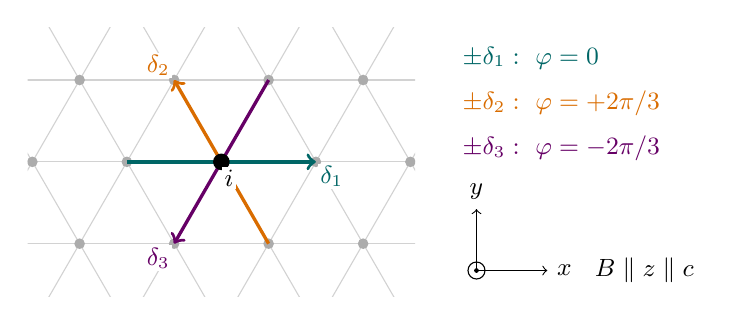
\begin{tikzpicture}[scale=1.2, font=\small]
  % Triangular Bravais lattice, adapted from the supplied source diagram.
  \begin{scope}
    \clip (-2.05,-1.42) rectangle (2.05,1.42);
    \foreach \m in {-4,...,4} {
      \foreach \n in {-3,...,3} {
        \coordinate (v) at ({\m-\n/2},{sqrt(3)*\n/2});
        \foreach \a in {0,60,120} {
          \draw[gray!35] (v)--++(\a:1);
        }
        \fill[gray!65] (v) circle (1.6pt);
      }
    }
  \end{scope}
  \draw[very thick,teal!80!black] (-1,0)--(0,0);
  \draw[very thick,orange!85!black] (300:1)--(0,0);
  \draw[very thick,violet!80!black] (60:1)--(0,0);
  \draw[->,very thick,teal!80!black] (0,0)--(0:1)
    node[below right,fill=white,inner sep=1pt] {\(\boldsymbol\delta_1\)};
  \draw[->,very thick,orange!85!black] (0,0)--(120:1)
    node[above left,fill=white,inner sep=1pt] {\(\boldsymbol\delta_2\)};
  \draw[->,very thick,violet!80!black] (0,0)--(240:1)
    node[below left,fill=white,inner sep=1pt] {\(\boldsymbol\delta_3\)};
  \fill[black] (0,0) circle (2.5pt);
  \node[below right,fill=white,inner sep=1pt] at (0,-0.05) {\(i\)};
  \node[anchor=west,teal!80!black] at (2.45,1.10)
    {\(\pm\boldsymbol\delta_1:\ \varphi=0\)};
  \node[anchor=west,orange!85!black] at (2.45,0.62)
    {\(\pm\boldsymbol\delta_2:\ \varphi=+2\pi/3\)};
  \node[anchor=west,violet!80!black] at (2.45,0.14)
    {\(\pm\boldsymbol\delta_3:\ \varphi=-2\pi/3\)};
  \begin{scope}[shift={(2.7,-1.15)}]
    \draw[->] (0,0)--(0.75,0) node[right] {\(x\)};
    \draw[->] (0,0)--(0,0.65) node[above] {\(y\)};
    \draw (0,0) circle (0.09);
    \fill (0,0) circle (0.025);
    \node[anchor=west] at (1.15,0) {\(B\parallel z\parallel c\)};
  \end{scope}
\end{tikzpicture}
\caption{Triangular lattice and nearest-neighbor vectors
\(\boldsymbol\delta_{1,2,3}\). Opposite bonds share the indicated phase;
\(\boldsymbol\delta_1\parallel x\). The dot-in-circle denotes a field
out of the plane.}
\label{fig-nbcp-bond-phases}
\end{figure}

\newpage
\subsection{Symmetries}\label{sec-nbcp-model-symmetry-properties}

The three terms have distinct symmetry properties~\cite{park2026}.
First, a nonzero perpendicular field reduces the unitary crystallographic
point group from \(\mathsf D_{3d}\) to \(\mathsf S_6\).
Second, the bond-dependent PD and \(\Gamma\) exchanges explicitly break
the global spin-\(z\) U(1) symmetry of \(H_{\rm XXZ}\), while preserving
\(\mathsf S_6\) under simultaneous transformations of lattice sites and
spins. In the paper's convention, a sixfold spatial rotation followed
by reflection in the layer acts on the axial spin as
\begin{equation}\label{eq-nbcp-s6-transform}
S_6:\quad
\hat S_j^x\pm i\hat S_j^y\longrightarrow
 e^{\mp i2\pi/3}(\hat S_{j'}^x\pm i\hat S_{j'}^y),
\qquad \hat S_j^z\longrightarrow\hat S_{j'}^z,
\end{equation}
where \(j'\) is the transformed lattice site. This combined symmetry
constrains the angular pinning discussed below; it is not a continuous
spin rotation at fixed lattice positions.

Third, a pure spin rotation \(U_\pi=\exp(-i\pi\sum_j\hat S_j^z)\)
leaves \(H_{\rm PD}\) invariant but sends \(H_\Gamma\) to
\(-H_\Gamma\). Thus nonzero \(J_\Gamma\) removes the additional
\(\pi\)-rotation symmetry retained by the XXZ+PD model.

\subsection{Parameters and conventions}\label{sec-nbcp-model-parameters}

For the Y/V gap comparison we use
\(J=0.075\,\mathrm{meV}\), \(J_z=0.125\,\mathrm{meV}\) and
\(g_z=4.645\), following Fig.~4 of Park et al.~\cite{park2026}.
The bond-dependent couplings and field are specified for each calculation.
Spin operators are dimensionless; exchange constants, \(h\) and gaps
are in meV, and \(e\) denotes energy per physical spin.
The exchange-model limit \(J_{\rm PD}=J_\Gamma=0\) does not remove the
atomic SOC that forms the effective doublet.
Historical parameter sets and the \(J=2J_\pm\) convention are given in
Appendix~\ref{app-nbcp-model-derivation}.
